\begin{figure}[h]
    \centering
    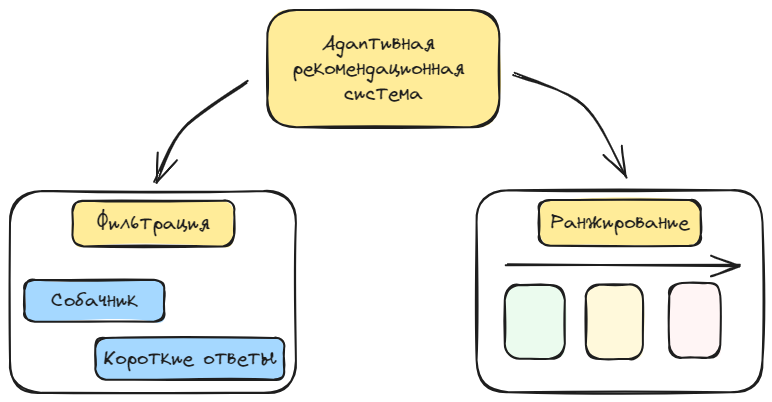
\includegraphics[width=0.5\textwidth]{assets/work/rating/bayes.excalidraw.png}
    \caption{Ht}
    \label{recommendation}
\end{figure}

Подход совмещающий использование ассистента совместно.
Существуют постановки, в которых вызов инструментов выполняется 

Таким образом, итоговый ассистент с
Совмещающий байесову рекомендательную систему как систему долгосрочного планирования и ассистента как эмпатического посредника.



Для адаптации открытой реализации для работы с детьми необходимо создание формата и предмета коммуникации.

Бранные слова были исключены с помощью библиотеки PyMorphy \cite{Korobov2015morph}, выделяющую нормальную форму слова для сравнения
с опорным корпусом неэтичных слов.

\begin{figure}[h]
    \centering
    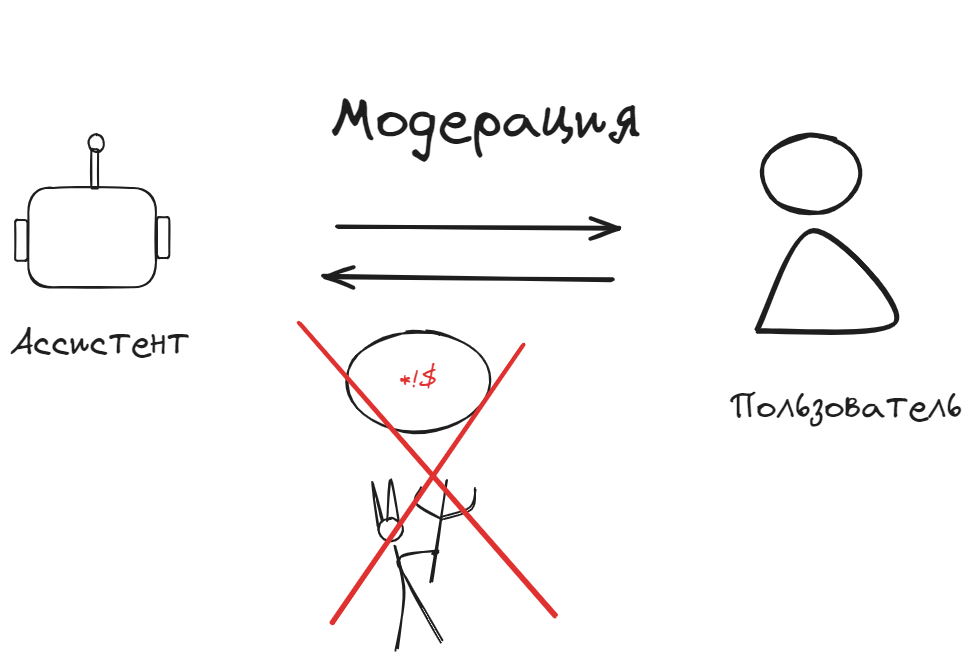
\includegraphics[width=0.5\textwidth]{assets/work/arch/detox.excalidraw.png}
    \caption{Модули PyMorphy \cite{Korobov2015morph} и CLIP позволяют исключить неэтичное общение и изображение }
    \label{detox}
\end{figure}




\begin{figure}[h]
    \centering
    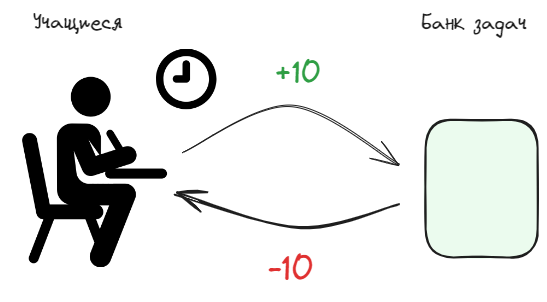
\includegraphics[width=0.5\textwidth]{assets/work/rating/recommendation.excalidraw.png}
    \caption{Проект приложения}
    \label{arch}
\end{figure}

Байесовы рейтинговые модели задают правила обновления апостериорных представлений рейтинга. Наиболее известным примером байесовой модели рейтинга является модель Брэдли-Терри и эквивалентная ей модель Эло.

Ключевым преимуществом байесовых систем является возможность пересчета рейтинга сразу после матча. Таким образом система приобретает адаптивность, важную в коммуникациях в настоящем времени.






В такой постановке ассистент следит за эмоциональным откликом обучающегося на материал,
узнает ее причину и в случае несоразмерной уровню нагрузке сообщает управляющей системе о потребности изменения сложности.

Плюсами такого подхода является \begin{itemize}
    \item интерпретируемость
    \item сужение ассистента до строгой постановки поиска наилучших навыков общения исходя из A/B тестирования.
\end{itemize}



